\setcounter{figure}{0}

\section{24th September 2023: The security of love}
\subsection*{Text: Song of Solomon 7:11-8:14}
  \begin{quote}
    [11] Come, my beloved,
        let us go out into the fields
        and lodge in the villages;
    [12] let us go out early to the vineyards
        and see whether the vines have budded,
    whether the grape blossoms have opened
        and the pomegranates are in bloom.
    There I will give you my love.
    [13] The mandrakes give forth fragrance,
        and beside our doors are all choice fruits,
    new as well as old,
        which I have laid up for you, O my beloved.


    [1] Oh that you were like a brother to me
        who nursed at my mother’s breasts!
    If I found you outside, I would kiss you,
        and none would despise me.
    [2] I would lead you and bring you
        into the house of my mother—
        she who used to teach me.
    I would give you spiced wine to drink,
        the juice of my pomegranate.
    [3] His left hand is under my head,
        and his right hand embraces me!
    [4] I adjure you, O daughters of Jerusalem,
        that you not stir up or awaken love
        until it pleases.


    [5] Who is that coming up from the wilderness,
        leaning on her beloved?


    Under the apple tree I awakened you.
    There your mother was in labor with you;
        there she who bore you was in labor.


    [6] Set me as a seal upon your heart,
        as a seal upon your arm,
    for love is strong as death,
        jealousy is fierce as the grave.
    Its flashes are flashes of fire,
        the very flame of the LORD.
    [7] Many waters cannot quench love,
        neither can floods drown it.
    If a man offered for love
        all the wealth of his house,
        he would be utterly despised.


        Others

    [8] We have a little sister,
        and she has no breasts.
    What shall we do for our sister
        on the day when she is spoken for?
    [9] If she is a wall,
        we will build on her a battlement of silver,
    but if she is a door,
        we will enclose her with boards of cedar.


    She

    [10] I was a wall,
        and my breasts were like towers;
    then I was in his eyes
        as one who finds peace.


    [11] Solomon had a vineyard at Baal-hamon;
        he let out the vineyard to keepers;
        each one was to bring for its fruit a thousand pieces of silver.
    [12] My vineyard, my very own, is before me;
        you, O Solomon, may have the thousand,
        and the keepers of the fruit two hundred.


    He

    [13] O you who dwell in the gardens,
        with companions listening for your voice;
        let me hear it.


    She

    [14] Make haste, my beloved,
        and be like a gazelle
    or a young stag
        on the mountains of spices.
  \end{quote}
\subsection*{Notes}
\begin{itemize}
  \item{Romantic love is something that is hard to explain. Romantic love is more than just a biological phenomenon caused by the release of hormones. When one’s spouse asks: “why do you love me?”, it is usually a difficult question to answer.}
  \item{That’s why God included the song of songs in the bible, to teach us romantic love through poetry that connects with out heart and teaches us love through our heart.}
  \item{Romantic love, like all forms of love (like the love between friends), moves us out of ourselves to commune with another. This is what we are made for, community. So there is a desire to love another, and there is a desire to be loved by another.}
  \item{In ch8 v1, the explanation is this: in the ancient world, PDA (public display of affection) is frowned upon. In v1 it is the woman saying that she loves her husband so much that she wishes it would not be taboo for them to PDA outside, such as would be the case if they were thought to be siblings. So in ch7:11-13 and in ch8:1-7, we see the woman showing her desire to show love to her husband and also to receive love from her husband.}
  \item{Now, love is “other-centred”, which is something that is difficult for us sinful humans to do, since sinful humans like us are “self-centred”. Hence, for us sinful humans, we can say that love is a virtue that needs to be cultivated (through the Holy Spirit).}
  \item{In the context of marital love, sex is supposed to be “other-centred”. And that is love. Sex is supposed to be self-giving, it is supposed to be a person giving of themselves to another person, it should be a person seeking the other person’s pleasure. On the other hand, lust is when the sexual desire is “self-centred”. In lustful sex, a person desires only his/her own pleasure, not the pleasure of his/her wife/husband. This is a perversion of sexual desire that God created. And pornography is an example of this.}
  \item{In the latter half of chapter 8 (v11-12), we see the man comparing his love with solomon’s love; the man’s love is “other centred”, it is centred on his wife’s welfare, whereas solomon’s love is “self centred”, it is centred on his own pleasure. This is why solomon had 1000 lovers, all to satisfy his lust, whereas the man only has one lover, his wife, because he seeks his wife’s welfare.}
  \item{Also in the later half of ch8 (v8-9), it is a description of the woman’s youth. When she was young, her family helped to adorn her (e.g, the metaphor of the wall/door and the adorning of the wall/door).  This is so the woman can attract a potential suitor. But in v10, the woman already doesn’t need her family’s help. This is because in v10, she already knows how to love, and she already knows she is loved by her husband. This is an example of maturity on the woman’s part; because she is loved by her husband, she knows how to love on her own without the help of her family. Similarly, when we know we are loved by God, that helps us to mature and know how to love. }
  \item{In v6-7, we see that the romantic love between husband and wife is exclusive and strong. This is the analogy which is used for God’s love for His people in the OT, such as in Hosea. }
  \item{Now, we note that ch8.14 ends very abruptly. But that might be the point: ``The effect of 8:14 is to assure us that the Song will never end, that the lovers will evermore be engaged in love's game of seeking and finding. The final words of the poem send us back to the beginning, to the voice that speaks in 1:2.''}
  \item{There is a longing/expectation for eternal love in song of songs itself. And this expectation for eternal love is found across all cultures.}
  \item{However, eternal love is not possible because of death. UNLESS, the love we are talking about is God’s love for us. While we might die, our death doesn’t separate us from God’s love for us. God’s love for us is STRONGER than the grave, FIERCER than death. Through life and death, God loves us. And, the christian fellowship and friendship that we share with each other will never end too; in the resurrection we’ll be like the angels, perfectly loving God and each other :).}
  \item{\begin{figure}[H]
    \centering
    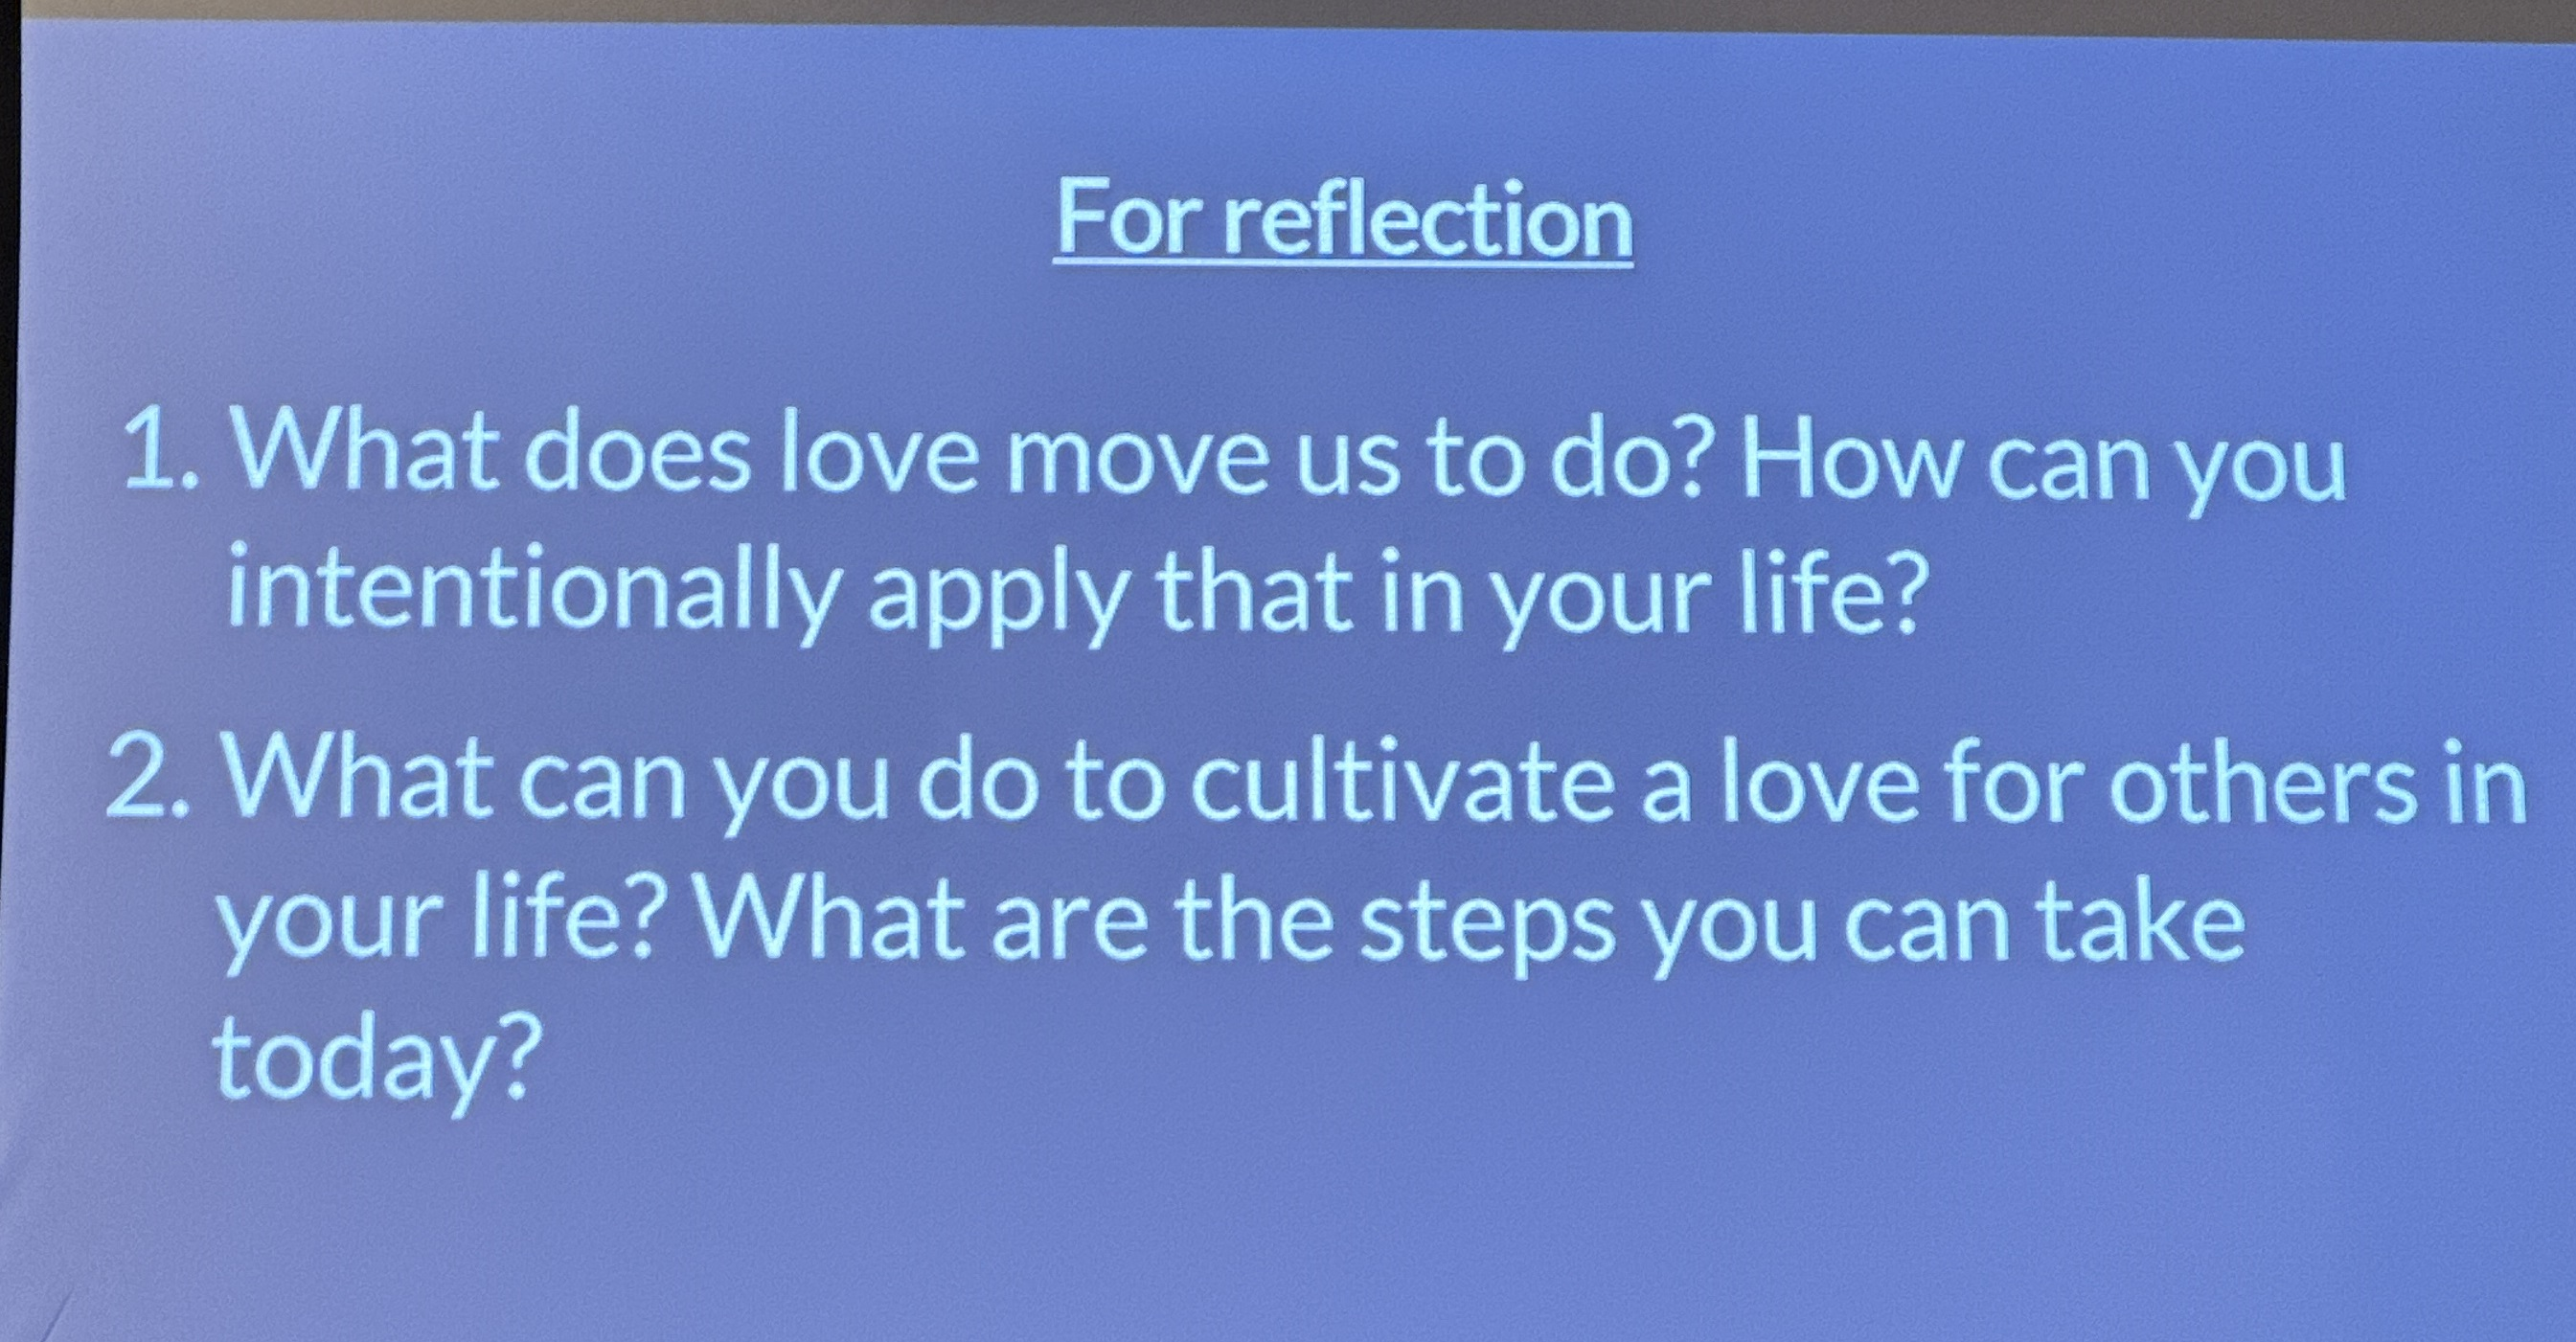
\includegraphics[width=0.8\textwidth, trim={0cm 0cm 0cm 0cm},clip]{Figures/septemberSermon4Reflections.jpg}
    % \includegraphics[width=0.8\textwidth, trim={0cm 0cm 0cm 0cm},clip]{example-image-a}
    \caption[]{Reflection questions for this sermon}
  \end{figure}}
\end{itemize}